\documentclass[a4paper,17pt]{extarticle}


    \usepackage[sfdefault, condensed]{roboto} % police d'écriture plus moderne
\usepackage[french]{babel} % francisation
\usepackage[parfill]{parskip} %suppression indentation

\usepackage{fancyhdr}
\usepackage{multicol}

% figure non flotantes
\usepackage{float}
\let\origfigure\figure
\let\endorigfigure\endfigure
\renewenvironment{figure}[1][2] {
    \expandafter\origfigure\expandafter[H]
} {
    \endorigfigure
}

% mois/année
\usepackage{datetime}
\newdateformat{monthyeardate}{%
  \monthname[\THEMONTH] \THEYEAR}

% couleurs perso
\usepackage[table]{xcolor}
\definecolor{deepblue}{rgb}{0.3,0.3,0.8}
\definecolor{darkblue}{rgb}{0,0,0.3}
\definecolor{deepred}{rgb}{0.6,0,0}
\definecolor{iremred}{RGB}{204,35,50}
\definecolor{deepgreen}{rgb}{0,0.6,0}
\definecolor{backcolor}{rgb}{0.98,0.95,0.95}
\definecolor{grisClair}{rgb}{0.95,0.95,0.95}
\definecolor{orangeamu}{RGB}{250,178,11}
\definecolor{noiramu}{RGB}{35,31,32}
\definecolor{bleuamu}{RGB}{20,118,198}
\definecolor{bleuamudark}{RGB}{15,90,150}
\definecolor{cyanamu}{RGB}{77,198,244}


\usepackage{/home/bouscadilla/Documents/Code/nbconvert/template/latex/pdf_solution/xeboiboites}
%
% exemple
\newbreakabletheorem[
    small box style={fill=deepblue!90,draw=deepblue!15, rounded corners,line width=1pt},%
    big box style={fill=deepblue!5,draw=deepblue!15,thick,rounded corners,line width=1pt},%
    headfont={\color{white}\bfseries}
        ]{exemple}{Exemple}{}%{counterCo}
%
% remarque
\newbreakabletheorem[
    small box style={draw=ansi-green-intense!100,line width=2pt,fill=ansi-green-intense!0,rounded corners,decoration=penciline, decorate},%
	big box style={color=ansi-green-intense!90,fill=ansi-green-intense!10,thick,decoration={penciline},decorate},
    broken edges={draw=ansi-green-intense!90,thick,fill=orange!20!black!5, decoration={random steps, segment length=.5cm,amplitude=1.3mm},decorate},%
    other edges={decoration=penciline,decorate,thick},%
    headfont={\color{ansi-green-intense}\large\scshape\bfseries}
    ]{remarque}{Remarque}{}%{counterCa}
%
% formule (sans titre)
\newboxedequation[%
    big box style={fill=cyanamu!10,draw=cyanamu!100,thick,decoration=penciline,decorate}]%
    {form}
%
% Réponse
\newbreakabletheorem[
    small box style={fill=bleuamu!100, draw=bleuamu!60, line width=1pt,rounded corners,decorate},%
    big box style={fill=bleuamu!10,draw=bleuamu!30,thick,rounded corners,decorate},
    headfont={\color{white}\large\scshape\bfseries}
        ]{reponse}{Correction}{}
%

%
% À retenir
%\newbreakabletheorem[
%    small box style={fill=deepred!100, draw=deepred!80, line width=1pt,rounded corners,decorate},%
%    big box style={fill=deepred!10,draw=deepred!50,thick,rounded corners,decorate},
%    headfont={\color{white}\large\scshape\bfseries}
%        ]{retenir}{À retenir}{}
%
\newboxedequation[%
    big box style={fill=deepred!10,draw=deepred!0,thick,decoration=penciline,decorate}]%
    {retenir}



% astuce
\newspanning[
    image=/home/bouscadilla/Documents/Code/nbconvert/template/latex/pdf_solution/fig-idee,headfont=\bfseries,
    spanning style={very thick,decoration=penciline,decorate}
    ]{astuce}{Astuce}{}
%
% activité

\newcounter{counterCa}
\newbreakabletheorem[
    small box style={draw=orangeamu!100,line width=2pt,fill=orangeamu!100,rounded corners,decoration=penciline, decorate},%
	big box style={color=orangeamu!100,fill=orangeamu!5,thick,decoration={penciline},decorate},
    broken edges={draw=orangeamu!100,thick,fill=orangeamu!100, decoration={random steps, segment length=.5cm,amplitude=1.3mm},decorate},%
    other edges={decoration=penciline,decorate,thick},%
    headfont={\color{white}\large\scshape\bfseries}
    ]{activite}{\adjustimage{height=1cm, valign=m}{/home/bouscadilla/Documents/Code/nbconvert/template/latex/pdf_solution/papier_eleve_investigation.png}%
    Activité}{counterCa}
%   
%   environnement élève
%
\newenvironment{eleve}%
%{\begin{activite}\large\\} % écrire plus gros
{\begin{activite}\color{noiramu}\\[-0.5cm]}
{\end{activite}}

\newenvironment{formule}%
%{\begin{activite}\large\\} % écrire plus gros
{\begin{form}\color{bleuamu}}
{\end{form}}


\usepackage[breakable]{tcolorbox}
    \usepackage{parskip} % Stop auto-indenting (to mimic markdown behaviour)
    
    \usepackage{iftex}
    \ifPDFTeX
    	\usepackage[T1]{fontenc}
    	\usepackage{mathpazo}
    \else
    	\usepackage{fontspec}
    \fi

    % Basic figure setup, for now with no caption control since it's done
    % automatically by Pandoc (which extracts ![](path) syntax from Markdown).
    \usepackage{graphicx}
    % Maintain compatibility with old templates. Remove in nbconvert 6.0
    \let\Oldincludegraphics\includegraphics
    % Ensure that by default, figures have no caption (until we provide a
    % proper Figure object with a Caption API and a way to capture that
    % in the conversion process - todo).
    \usepackage{caption}
    \DeclareCaptionFormat{nocaption}{}
    \captionsetup{format=nocaption,aboveskip=0pt,belowskip=0pt}

    \usepackage[Export]{adjustbox} % Used to constrain images to a maximum size
    \adjustboxset{max size={0.9\linewidth}{0.9\paperheight}}
    \usepackage{float}
    \floatplacement{figure}{H} % forces figures to be placed at the correct location
    \usepackage{xcolor} % Allow colors to be defined
    \usepackage{enumerate} % Needed for markdown enumerations to work
    \usepackage{geometry} % Used to adjust the document margins
    \usepackage{amsmath} % Equations
    \usepackage{amssymb} % Equations
    \usepackage{textcomp} % defines textquotesingle
    % Hack from http://tex.stackexchange.com/a/47451/13684:
    \AtBeginDocument{%
        \def\PYZsq{\textquotesingle}% Upright quotes in Pygmentized code
    }
    \usepackage{upquote} % Upright quotes for verbatim code
    \usepackage{eurosym} % defines \euro
    \usepackage[mathletters]{ucs} % Extended unicode (utf-8) support
    \usepackage{fancyvrb} % verbatim replacement that allows latex

    % The hyperref package gives us a pdf with properly built
    % internal navigation ('pdf bookmarks' for the table of contents,
    % internal cross-reference links, web links for URLs, etc.)
    \usepackage{hyperref}
    % The default LaTeX title has an obnoxious amount of whitespace. By default,
    % titling removes some of it. It also provides customization options.
    \usepackage{titling}
    \usepackage{longtable} % longtable support required by pandoc >1.10
    \usepackage{booktabs}  % table support for pandoc > 1.12.2
    \usepackage[inline]{enumitem} % IRkernel/repr support (it uses the enumerate* environment)
    \usepackage[normalem]{ulem} % ulem is needed to support strikethroughs (\sout)
                                % normalem makes italics be italics, not underlines
    \usepackage{mathrsfs}
    

    
    % Colors for the hyperref package
    \definecolor{urlcolor}{rgb}{0,.145,.698}
    \definecolor{linkcolor}{rgb}{.71,0.21,0.01}
    \definecolor{citecolor}{rgb}{.12,.54,.11}

    % ANSI colors
    \definecolor{ansi-black}{HTML}{3E424D}
    \definecolor{ansi-black-intense}{HTML}{282C36}
    \definecolor{ansi-red}{HTML}{E75C58}
    \definecolor{ansi-red-intense}{HTML}{B22B31}
    \definecolor{ansi-green}{HTML}{00A250}
    \definecolor{ansi-green-intense}{HTML}{007427}
    \definecolor{ansi-yellow}{HTML}{DDB62B}
    \definecolor{ansi-yellow-intense}{HTML}{B27D12}
    \definecolor{ansi-blue}{HTML}{208FFB}
    \definecolor{ansi-blue-intense}{HTML}{0065CA}
    \definecolor{ansi-magenta}{HTML}{D160C4}
    \definecolor{ansi-magenta-intense}{HTML}{A03196}
    \definecolor{ansi-cyan}{HTML}{60C6C8}
    \definecolor{ansi-cyan-intense}{HTML}{258F8F}
    \definecolor{ansi-white}{HTML}{C5C1B4}
    \definecolor{ansi-white-intense}{HTML}{A1A6B2}
    \definecolor{ansi-default-inverse-fg}{HTML}{FFFFFF}
    \definecolor{ansi-default-inverse-bg}{HTML}{000000}

    % commands and environments needed by pandoc snippets
    % extracted from the output of `pandoc -s`
    \providecommand{\tightlist}{%
      \setlength{\itemsep}{0pt}\setlength{\parskip}{0pt}}
    \DefineVerbatimEnvironment{Highlighting}{Verbatim}{commandchars=\\\{\}}
    % Add ',fontsize=\small' for more characters per line
    \newenvironment{Shaded}{}{}
    \newcommand{\KeywordTok}[1]{\textcolor[rgb]{0.00,0.44,0.13}{\textbf{{#1}}}}
    \newcommand{\DataTypeTok}[1]{\textcolor[rgb]{0.56,0.13,0.00}{{#1}}}
    \newcommand{\DecValTok}[1]{\textcolor[rgb]{0.25,0.63,0.44}{{#1}}}
    \newcommand{\BaseNTok}[1]{\textcolor[rgb]{0.25,0.63,0.44}{{#1}}}
    \newcommand{\FloatTok}[1]{\textcolor[rgb]{0.25,0.63,0.44}{{#1}}}
    \newcommand{\CharTok}[1]{\textcolor[rgb]{0.25,0.44,0.63}{{#1}}}
    \newcommand{\StringTok}[1]{\textcolor[rgb]{0.25,0.44,0.63}{{#1}}}
    \newcommand{\CommentTok}[1]{\textcolor[rgb]{0.38,0.63,0.69}{\textit{{#1}}}}
    \newcommand{\OtherTok}[1]{\textcolor[rgb]{0.00,0.44,0.13}{{#1}}}
    \newcommand{\AlertTok}[1]{\textcolor[rgb]{1.00,0.00,0.00}{\textbf{{#1}}}}
    \newcommand{\FunctionTok}[1]{\textcolor[rgb]{0.02,0.16,0.49}{{#1}}}
    \newcommand{\RegionMarkerTok}[1]{{#1}}
    \newcommand{\ErrorTok}[1]{\textcolor[rgb]{1.00,0.00,0.00}{\textbf{{#1}}}}
    \newcommand{\NormalTok}[1]{{#1}}
    
    % Additional commands for more recent versions of Pandoc
    \newcommand{\ConstantTok}[1]{\textcolor[rgb]{0.53,0.00,0.00}{{#1}}}
    \newcommand{\SpecialCharTok}[1]{\textcolor[rgb]{0.25,0.44,0.63}{{#1}}}
    \newcommand{\VerbatimStringTok}[1]{\textcolor[rgb]{0.25,0.44,0.63}{{#1}}}
    \newcommand{\SpecialStringTok}[1]{\textcolor[rgb]{0.73,0.40,0.53}{{#1}}}
    \newcommand{\ImportTok}[1]{{#1}}
    \newcommand{\DocumentationTok}[1]{\textcolor[rgb]{0.73,0.13,0.13}{\textit{{#1}}}}
    \newcommand{\AnnotationTok}[1]{\textcolor[rgb]{0.38,0.63,0.69}{\textbf{\textit{{#1}}}}}
    \newcommand{\CommentVarTok}[1]{\textcolor[rgb]{0.38,0.63,0.69}{\textbf{\textit{{#1}}}}}
    \newcommand{\VariableTok}[1]{\textcolor[rgb]{0.10,0.09,0.49}{{#1}}}
    \newcommand{\ControlFlowTok}[1]{\textcolor[rgb]{0.00,0.44,0.13}{\textbf{{#1}}}}
    \newcommand{\OperatorTok}[1]{\textcolor[rgb]{0.40,0.40,0.40}{{#1}}}
    \newcommand{\BuiltInTok}[1]{{#1}}
    \newcommand{\ExtensionTok}[1]{{#1}}
    \newcommand{\PreprocessorTok}[1]{\textcolor[rgb]{0.74,0.48,0.00}{{#1}}}
    \newcommand{\AttributeTok}[1]{\textcolor[rgb]{0.49,0.56,0.16}{{#1}}}
    \newcommand{\InformationTok}[1]{\textcolor[rgb]{0.38,0.63,0.69}{\textbf{\textit{{#1}}}}}
    \newcommand{\WarningTok}[1]{\textcolor[rgb]{0.38,0.63,0.69}{\textbf{\textit{{#1}}}}}
    
    
    % Define a nice break command that doesn't care if a line doesn't already
    % exist.
    \def\br{\hspace*{\fill} \\* }
    % Math Jax compatibility definitions
    \def\gt{>}
    \def\lt{<}
    \let\Oldtex\TeX
    \let\Oldlatex\LaTeX
    \renewcommand{\TeX}{\textrm{\Oldtex}}
    \renewcommand{\LaTeX}{\textrm{\Oldlatex}}
    % Document parameters
    % Document title
    \title{5-4---ListesChainees-encapsulation}
    
    
    
    
    
% Pygments definitions
\makeatletter
\def\PY@reset{\let\PY@it=\relax \let\PY@bf=\relax%
    \let\PY@ul=\relax \let\PY@tc=\relax%
    \let\PY@bc=\relax \let\PY@ff=\relax}
\def\PY@tok#1{\csname PY@tok@#1\endcsname}
\def\PY@toks#1+{\ifx\relax#1\empty\else%
    \PY@tok{#1}\expandafter\PY@toks\fi}
\def\PY@do#1{\PY@bc{\PY@tc{\PY@ul{%
    \PY@it{\PY@bf{\PY@ff{#1}}}}}}}
\def\PY#1#2{\PY@reset\PY@toks#1+\relax+\PY@do{#2}}

\expandafter\def\csname PY@tok@w\endcsname{\def\PY@tc##1{\textcolor[rgb]{0.73,0.73,0.73}{##1}}}
\expandafter\def\csname PY@tok@c\endcsname{\let\PY@it=\textit\def\PY@tc##1{\textcolor[rgb]{0.25,0.50,0.50}{##1}}}
\expandafter\def\csname PY@tok@cp\endcsname{\def\PY@tc##1{\textcolor[rgb]{0.74,0.48,0.00}{##1}}}
\expandafter\def\csname PY@tok@k\endcsname{\let\PY@bf=\textbf\def\PY@tc##1{\textcolor[rgb]{0.00,0.50,0.00}{##1}}}
\expandafter\def\csname PY@tok@kp\endcsname{\def\PY@tc##1{\textcolor[rgb]{0.00,0.50,0.00}{##1}}}
\expandafter\def\csname PY@tok@kt\endcsname{\def\PY@tc##1{\textcolor[rgb]{0.69,0.00,0.25}{##1}}}
\expandafter\def\csname PY@tok@o\endcsname{\def\PY@tc##1{\textcolor[rgb]{0.40,0.40,0.40}{##1}}}
\expandafter\def\csname PY@tok@ow\endcsname{\let\PY@bf=\textbf\def\PY@tc##1{\textcolor[rgb]{0.67,0.13,1.00}{##1}}}
\expandafter\def\csname PY@tok@nb\endcsname{\def\PY@tc##1{\textcolor[rgb]{0.00,0.50,0.00}{##1}}}
\expandafter\def\csname PY@tok@nf\endcsname{\def\PY@tc##1{\textcolor[rgb]{0.00,0.00,1.00}{##1}}}
\expandafter\def\csname PY@tok@nc\endcsname{\let\PY@bf=\textbf\def\PY@tc##1{\textcolor[rgb]{0.00,0.00,1.00}{##1}}}
\expandafter\def\csname PY@tok@nn\endcsname{\let\PY@bf=\textbf\def\PY@tc##1{\textcolor[rgb]{0.00,0.00,1.00}{##1}}}
\expandafter\def\csname PY@tok@ne\endcsname{\let\PY@bf=\textbf\def\PY@tc##1{\textcolor[rgb]{0.82,0.25,0.23}{##1}}}
\expandafter\def\csname PY@tok@nv\endcsname{\def\PY@tc##1{\textcolor[rgb]{0.10,0.09,0.49}{##1}}}
\expandafter\def\csname PY@tok@no\endcsname{\def\PY@tc##1{\textcolor[rgb]{0.53,0.00,0.00}{##1}}}
\expandafter\def\csname PY@tok@nl\endcsname{\def\PY@tc##1{\textcolor[rgb]{0.63,0.63,0.00}{##1}}}
\expandafter\def\csname PY@tok@ni\endcsname{\let\PY@bf=\textbf\def\PY@tc##1{\textcolor[rgb]{0.60,0.60,0.60}{##1}}}
\expandafter\def\csname PY@tok@na\endcsname{\def\PY@tc##1{\textcolor[rgb]{0.49,0.56,0.16}{##1}}}
\expandafter\def\csname PY@tok@nt\endcsname{\let\PY@bf=\textbf\def\PY@tc##1{\textcolor[rgb]{0.00,0.50,0.00}{##1}}}
\expandafter\def\csname PY@tok@nd\endcsname{\def\PY@tc##1{\textcolor[rgb]{0.67,0.13,1.00}{##1}}}
\expandafter\def\csname PY@tok@s\endcsname{\def\PY@tc##1{\textcolor[rgb]{0.73,0.13,0.13}{##1}}}
\expandafter\def\csname PY@tok@sd\endcsname{\let\PY@it=\textit\def\PY@tc##1{\textcolor[rgb]{0.73,0.13,0.13}{##1}}}
\expandafter\def\csname PY@tok@si\endcsname{\let\PY@bf=\textbf\def\PY@tc##1{\textcolor[rgb]{0.73,0.40,0.53}{##1}}}
\expandafter\def\csname PY@tok@se\endcsname{\let\PY@bf=\textbf\def\PY@tc##1{\textcolor[rgb]{0.73,0.40,0.13}{##1}}}
\expandafter\def\csname PY@tok@sr\endcsname{\def\PY@tc##1{\textcolor[rgb]{0.73,0.40,0.53}{##1}}}
\expandafter\def\csname PY@tok@ss\endcsname{\def\PY@tc##1{\textcolor[rgb]{0.10,0.09,0.49}{##1}}}
\expandafter\def\csname PY@tok@sx\endcsname{\def\PY@tc##1{\textcolor[rgb]{0.00,0.50,0.00}{##1}}}
\expandafter\def\csname PY@tok@m\endcsname{\def\PY@tc##1{\textcolor[rgb]{0.40,0.40,0.40}{##1}}}
\expandafter\def\csname PY@tok@gh\endcsname{\let\PY@bf=\textbf\def\PY@tc##1{\textcolor[rgb]{0.00,0.00,0.50}{##1}}}
\expandafter\def\csname PY@tok@gu\endcsname{\let\PY@bf=\textbf\def\PY@tc##1{\textcolor[rgb]{0.50,0.00,0.50}{##1}}}
\expandafter\def\csname PY@tok@gd\endcsname{\def\PY@tc##1{\textcolor[rgb]{0.63,0.00,0.00}{##1}}}
\expandafter\def\csname PY@tok@gi\endcsname{\def\PY@tc##1{\textcolor[rgb]{0.00,0.63,0.00}{##1}}}
\expandafter\def\csname PY@tok@gr\endcsname{\def\PY@tc##1{\textcolor[rgb]{1.00,0.00,0.00}{##1}}}
\expandafter\def\csname PY@tok@ge\endcsname{\let\PY@it=\textit}
\expandafter\def\csname PY@tok@gs\endcsname{\let\PY@bf=\textbf}
\expandafter\def\csname PY@tok@gp\endcsname{\let\PY@bf=\textbf\def\PY@tc##1{\textcolor[rgb]{0.00,0.00,0.50}{##1}}}
\expandafter\def\csname PY@tok@go\endcsname{\def\PY@tc##1{\textcolor[rgb]{0.53,0.53,0.53}{##1}}}
\expandafter\def\csname PY@tok@gt\endcsname{\def\PY@tc##1{\textcolor[rgb]{0.00,0.27,0.87}{##1}}}
\expandafter\def\csname PY@tok@err\endcsname{\def\PY@bc##1{\setlength{\fboxsep}{0pt}\fcolorbox[rgb]{1.00,0.00,0.00}{1,1,1}{\strut ##1}}}
\expandafter\def\csname PY@tok@kc\endcsname{\let\PY@bf=\textbf\def\PY@tc##1{\textcolor[rgb]{0.00,0.50,0.00}{##1}}}
\expandafter\def\csname PY@tok@kd\endcsname{\let\PY@bf=\textbf\def\PY@tc##1{\textcolor[rgb]{0.00,0.50,0.00}{##1}}}
\expandafter\def\csname PY@tok@kn\endcsname{\let\PY@bf=\textbf\def\PY@tc##1{\textcolor[rgb]{0.00,0.50,0.00}{##1}}}
\expandafter\def\csname PY@tok@kr\endcsname{\let\PY@bf=\textbf\def\PY@tc##1{\textcolor[rgb]{0.00,0.50,0.00}{##1}}}
\expandafter\def\csname PY@tok@bp\endcsname{\def\PY@tc##1{\textcolor[rgb]{0.00,0.50,0.00}{##1}}}
\expandafter\def\csname PY@tok@fm\endcsname{\def\PY@tc##1{\textcolor[rgb]{0.00,0.00,1.00}{##1}}}
\expandafter\def\csname PY@tok@vc\endcsname{\def\PY@tc##1{\textcolor[rgb]{0.10,0.09,0.49}{##1}}}
\expandafter\def\csname PY@tok@vg\endcsname{\def\PY@tc##1{\textcolor[rgb]{0.10,0.09,0.49}{##1}}}
\expandafter\def\csname PY@tok@vi\endcsname{\def\PY@tc##1{\textcolor[rgb]{0.10,0.09,0.49}{##1}}}
\expandafter\def\csname PY@tok@vm\endcsname{\def\PY@tc##1{\textcolor[rgb]{0.10,0.09,0.49}{##1}}}
\expandafter\def\csname PY@tok@sa\endcsname{\def\PY@tc##1{\textcolor[rgb]{0.73,0.13,0.13}{##1}}}
\expandafter\def\csname PY@tok@sb\endcsname{\def\PY@tc##1{\textcolor[rgb]{0.73,0.13,0.13}{##1}}}
\expandafter\def\csname PY@tok@sc\endcsname{\def\PY@tc##1{\textcolor[rgb]{0.73,0.13,0.13}{##1}}}
\expandafter\def\csname PY@tok@dl\endcsname{\def\PY@tc##1{\textcolor[rgb]{0.73,0.13,0.13}{##1}}}
\expandafter\def\csname PY@tok@s2\endcsname{\def\PY@tc##1{\textcolor[rgb]{0.73,0.13,0.13}{##1}}}
\expandafter\def\csname PY@tok@sh\endcsname{\def\PY@tc##1{\textcolor[rgb]{0.73,0.13,0.13}{##1}}}
\expandafter\def\csname PY@tok@s1\endcsname{\def\PY@tc##1{\textcolor[rgb]{0.73,0.13,0.13}{##1}}}
\expandafter\def\csname PY@tok@mb\endcsname{\def\PY@tc##1{\textcolor[rgb]{0.40,0.40,0.40}{##1}}}
\expandafter\def\csname PY@tok@mf\endcsname{\def\PY@tc##1{\textcolor[rgb]{0.40,0.40,0.40}{##1}}}
\expandafter\def\csname PY@tok@mh\endcsname{\def\PY@tc##1{\textcolor[rgb]{0.40,0.40,0.40}{##1}}}
\expandafter\def\csname PY@tok@mi\endcsname{\def\PY@tc##1{\textcolor[rgb]{0.40,0.40,0.40}{##1}}}
\expandafter\def\csname PY@tok@il\endcsname{\def\PY@tc##1{\textcolor[rgb]{0.40,0.40,0.40}{##1}}}
\expandafter\def\csname PY@tok@mo\endcsname{\def\PY@tc##1{\textcolor[rgb]{0.40,0.40,0.40}{##1}}}
\expandafter\def\csname PY@tok@ch\endcsname{\let\PY@it=\textit\def\PY@tc##1{\textcolor[rgb]{0.25,0.50,0.50}{##1}}}
\expandafter\def\csname PY@tok@cm\endcsname{\let\PY@it=\textit\def\PY@tc##1{\textcolor[rgb]{0.25,0.50,0.50}{##1}}}
\expandafter\def\csname PY@tok@cpf\endcsname{\let\PY@it=\textit\def\PY@tc##1{\textcolor[rgb]{0.25,0.50,0.50}{##1}}}
\expandafter\def\csname PY@tok@c1\endcsname{\let\PY@it=\textit\def\PY@tc##1{\textcolor[rgb]{0.25,0.50,0.50}{##1}}}
\expandafter\def\csname PY@tok@cs\endcsname{\let\PY@it=\textit\def\PY@tc##1{\textcolor[rgb]{0.25,0.50,0.50}{##1}}}

\def\PYZbs{\char`\\}
\def\PYZus{\char`\_}
\def\PYZob{\char`\{}
\def\PYZcb{\char`\}}
\def\PYZca{\char`\^}
\def\PYZam{\char`\&}
\def\PYZlt{\char`\<}
\def\PYZgt{\char`\>}
\def\PYZsh{\char`\#}
\def\PYZpc{\char`\%}
\def\PYZdl{\char`\$}
\def\PYZhy{\char`\-}
\def\PYZsq{\char`\'}
\def\PYZdq{\char`\"}
\def\PYZti{\char`\~}
% for compatibility with earlier versions
\def\PYZat{@}
\def\PYZlb{[}
\def\PYZrb{]}
\makeatother


    % For linebreaks inside Verbatim environment from package fancyvrb. 
    \makeatletter
        \newbox\Wrappedcontinuationbox 
        \newbox\Wrappedvisiblespacebox 
        \newcommand*\Wrappedvisiblespace {\textcolor{red}{\textvisiblespace}} 
        \newcommand*\Wrappedcontinuationsymbol {\textcolor{red}{\llap{\tiny$\m@th\hookrightarrow$}}} 
        \newcommand*\Wrappedcontinuationindent {3ex } 
        \newcommand*\Wrappedafterbreak {\kern\Wrappedcontinuationindent\copy\Wrappedcontinuationbox} 
        % Take advantage of the already applied Pygments mark-up to insert 
        % potential linebreaks for TeX processing. 
        %        {, <, #, %, $, ' and ": go to next line. 
        %        _, }, ^, &, >, - and ~: stay at end of broken line. 
        % Use of \textquotesingle for straight quote. 
        \newcommand*\Wrappedbreaksatspecials {% 
            \def\PYGZus{\discretionary{\char`\_}{\Wrappedafterbreak}{\char`\_}}% 
            \def\PYGZob{\discretionary{}{\Wrappedafterbreak\char`\{}{\char`\{}}% 
            \def\PYGZcb{\discretionary{\char`\}}{\Wrappedafterbreak}{\char`\}}}% 
            \def\PYGZca{\discretionary{\char`\^}{\Wrappedafterbreak}{\char`\^}}% 
            \def\PYGZam{\discretionary{\char`\&}{\Wrappedafterbreak}{\char`\&}}% 
            \def\PYGZlt{\discretionary{}{\Wrappedafterbreak\char`\<}{\char`\<}}% 
            \def\PYGZgt{\discretionary{\char`\>}{\Wrappedafterbreak}{\char`\>}}% 
            \def\PYGZsh{\discretionary{}{\Wrappedafterbreak\char`\#}{\char`\#}}% 
            \def\PYGZpc{\discretionary{}{\Wrappedafterbreak\char`\%}{\char`\%}}% 
            \def\PYGZdl{\discretionary{}{\Wrappedafterbreak\char`\$}{\char`\$}}% 
            \def\PYGZhy{\discretionary{\char`\-}{\Wrappedafterbreak}{\char`\-}}% 
            \def\PYGZsq{\discretionary{}{\Wrappedafterbreak\textquotesingle}{\textquotesingle}}% 
            \def\PYGZdq{\discretionary{}{\Wrappedafterbreak\char`\"}{\char`\"}}% 
            \def\PYGZti{\discretionary{\char`\~}{\Wrappedafterbreak}{\char`\~}}% 
        } 
        % Some characters . , ; ? ! / are not pygmentized. 
        % This macro makes them "active" and they will insert potential linebreaks 
        \newcommand*\Wrappedbreaksatpunct {% 
            \lccode`\~`\.\lowercase{\def~}{\discretionary{\hbox{\char`\.}}{\Wrappedafterbreak}{\hbox{\char`\.}}}% 
            \lccode`\~`\,\lowercase{\def~}{\discretionary{\hbox{\char`\,}}{\Wrappedafterbreak}{\hbox{\char`\,}}}% 
            \lccode`\~`\;\lowercase{\def~}{\discretionary{\hbox{\char`\;}}{\Wrappedafterbreak}{\hbox{\char`\;}}}% 
            \lccode`\~`\:\lowercase{\def~}{\discretionary{\hbox{\char`\:}}{\Wrappedafterbreak}{\hbox{\char`\:}}}% 
            \lccode`\~`\?\lowercase{\def~}{\discretionary{\hbox{\char`\?}}{\Wrappedafterbreak}{\hbox{\char`\?}}}% 
            \lccode`\~`\!\lowercase{\def~}{\discretionary{\hbox{\char`\!}}{\Wrappedafterbreak}{\hbox{\char`\!}}}% 
            \lccode`\~`\/\lowercase{\def~}{\discretionary{\hbox{\char`\/}}{\Wrappedafterbreak}{\hbox{\char`\/}}}% 
            \catcode`\.\active
            \catcode`\,\active 
            \catcode`\;\active
            \catcode`\:\active
            \catcode`\?\active
            \catcode`\!\active
            \catcode`\/\active 
            \lccode`\~`\~ 	
        }
    \makeatother

    \let\OriginalVerbatim=\Verbatim
    \makeatletter
    \renewcommand{\Verbatim}[1][1]{%
        %\parskip\z@skip
        \sbox\Wrappedcontinuationbox {\Wrappedcontinuationsymbol}%
        \sbox\Wrappedvisiblespacebox {\FV@SetupFont\Wrappedvisiblespace}%
        \def\FancyVerbFormatLine ##1{\hsize\linewidth
            \vtop{\raggedright\hyphenpenalty\z@\exhyphenpenalty\z@
                \doublehyphendemerits\z@\finalhyphendemerits\z@
                \strut ##1\strut}%
        }%
        % If the linebreak is at a space, the latter will be displayed as visible
        % space at end of first line, and a continuation symbol starts next line.
        % Stretch/shrink are however usually zero for typewriter font.
        \def\FV@Space {%
            \nobreak\hskip\z@ plus\fontdimen3\font minus\fontdimen4\font
            \discretionary{\copy\Wrappedvisiblespacebox}{\Wrappedafterbreak}
            {\kern\fontdimen2\font}%
        }%
        
        % Allow breaks at special characters using \PYG... macros.
        \Wrappedbreaksatspecials
        % Breaks at punctuation characters . , ; ? ! and / need catcode=\active 	
        \OriginalVerbatim[#1,codes*=\Wrappedbreaksatpunct]%
    }
    \makeatother

    % Exact colors from NB
    \definecolor{incolor}{HTML}{303F9F}
    \definecolor{outcolor}{HTML}{D84315}
    \definecolor{cellborder}{HTML}{CFCFCF}
    \definecolor{cellbackground}{HTML}{F7F7F7}
    
    % prompt
    \makeatletter
    \newcommand{\boxspacing}{\kern\kvtcb@left@rule\kern\kvtcb@boxsep}
    \makeatother
    \newcommand{\prompt}[4]{
        \ttfamily\llap{{\color{#2}[#3]:\hspace{3pt}#4}}\vspace{-\baselineskip}
    }
    

    
\setlength\headheight{30pt}
\setcounter{secnumdepth}{0} % Turns off numbering for sections

    % Prevent overflowing lines due to hard-to-break entities
    \sloppy 
    % Setup hyperref package
    \hypersetup{
      breaklinks=true,  % so long urls are correctly broken across lines
      colorlinks=true,
      urlcolor=urlcolor,
      linkcolor=linkcolor,
      citecolor=citecolor,
      }
    % Slightly bigger margins than the latex defaults
    \geometry{a4paper,tmargin=3cm,bmargin=2cm,lmargin=1cm,rmargin=1cm}\fancyhead[L]{Thème à définir}\fancyhead[L]{\adjustimage{height=1cm, valign=m}{/home/bouscadilla/Documents/Code/nbconvert/template/latex/pdf_solution/papier_eleve_ico_structure}\ttfamily\scshape Struct.de données}\fancyhead[C]{\bfseries\MakeUppercase{5-4---ListesChainees-encapsulation}}\fancyhead[C]{\bfseries\MakeUppercase{5 --- Listes chaînées}}\fancyhead[R]{\monthyeardate\today}

    \fancyfoot[C]{\thepage}
    % #TODO ajouter les pages totales

    \pagestyle{fancy}
    


\begin{document}
    
    \title{5 --- Listes chaînées}
% \maketitle

    
    

    
    \hypertarget{encapsulation-dans-un-objet}{%
\subsection{4 --- Encapsulation dans un
objet}\label{encapsulation-dans-un-objet}}

    \hypertarget{muxe9thodes-de-bases}{%
\subsubsection{Méthodes de bases}\label{muxe9thodes-de-bases}}
\begin{retenir}
    Pour finir nous allons maintenant encapsuler une liste chaînée
\textbf{dans un objet}.

L'idée consiste à définir une nouvelle classe, \texttt{Liste}, qui
possède un unique attribut, \texttt{tete}, qui contient une liste
chaînée. On l'appelle tete car il désigne la tête de la liste, lorsque
celle-ci n'est pas vide (et \texttt{None} sinon). Le constructeur
initialise l'attribut \texttt{tete} avec la valeur \texttt{None}.

        \end{retenir}
    \begin{figure}
\centering
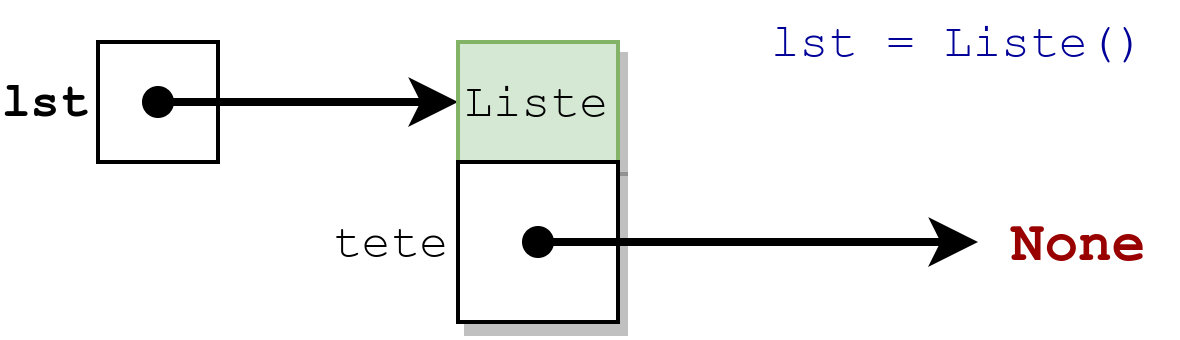
\includegraphics{maillon6.png}
\caption{constructeur de Liste()}
\end{figure}

    Il y a de multiples intérêts à cette encapsulation :

\begin{itemize}
\tightlist
\item
  D'une part, il cache la représentation de la structure à
  l'utilisateur. Ainsi, celui qui utilise notre classe \texttt{Liste}
  n'a plus à manipuler explicitement la classe \texttt{Maillon}. Mieux
  encore, il peut complètement ignorer son existence. De même, il ignore
  que la liste vide est représentée par la valeur \texttt{None}. En
  particulier, la réalisation de la classe \texttt{Liste} pourrait être
  modifiée sans pour autant que le code qui l'utilise n'ait besoin
  d'être modifié à son tour.
\item
  D'autre part, l'utilisation de classes et de méthodes nous permet de
  donner le même nom à toutes les méthodes qui sont de même nature.
  Ainsi, on peut avoir plusieurs classes avec des méthodes
  \texttt{est\_vide}, \texttt{ajoute}, etc. Si nous avions utilisé de
  simples fonctions, il faudrait distinguer \texttt{liste\_est\_vide},
  \texttt{pile\_est\_vide}, \texttt{ensemble\_est\_vide}, etc.
\end{itemize}
\begin{eleve}
    Implémenter la classe \texttt{Liste} avec un constructeur qui initialise
l'attribut \texttt{tete} à None.

Exemple :

\begin{verbatim}
>>> lst = Liste()
>>> print(lst.tete)
None
\end{verbatim}
        
        \end{eleve}
        {\scriptsize
    \begin{tcolorbox}[breakable, size=fbox, boxrule=1pt, pad at break*=1mm,colback=cellbackground, colframe=cellborder]
\prompt{In}{incolor}{ }{\boxspacing}
\begin{Verbatim}[commandchars=\\\{\}]
\PY{k}{class} \PY{n+nc}{Liste}\PY{p}{:}
    \PY{k}{def} \PY{n+nf+fm}{\PYZus{}\PYZus{}init\PYZus{}\PYZus{}}\PY{p}{(}\PY{n+nb+bp}{self}\PY{p}{)}\PY{p}{:}
        \PY{l+s+sd}{\PYZdq{}\PYZdq{}\PYZdq{}}
\PY{l+s+sd}{        Constructeur d\PYZsq{}une liste vide.}

\PY{l+s+sd}{        Exemples :}
\PY{l+s+sd}{        \PYZgt{}\PYZgt{}\PYZgt{} lst = Liste()}
\PY{l+s+sd}{        \PYZgt{}\PYZgt{}\PYZgt{} print(lst.tete)}
\PY{l+s+sd}{        None}
\PY{l+s+sd}{        \PYZdq{}\PYZdq{}\PYZdq{}}

        \PY{n+nb+bp}{self}\PY{o}{.}\PY{n}{tete} \PY{o}{=} \PY{k+kc}{None}


\PY{c+c1}{\PYZsh{} test avec l\PYZsq{}exemple}
\PY{n}{testmod}\PY{p}{(}\PY{p}{)}
\end{Verbatim}
\end{tcolorbox}
    }

    Ainsi, un objet construit avec \texttt{Liste()} représente une liste
vide.

On peut également introduire une méthode \texttt{est\_vide} qui renvoie
un booléen indiquant si la liste est vide. En effet, notre intention est
d'encapsuler, c'est-à-dire de cacher, la représentation de la liste
derrière cet objet. Pour cette raison, on n e souhaite pas que
l'utilisateur de la classe \texttt{Liste} teste explicitement si
l'attribut \texttt{tete} vaut \texttt{None}, mais qu'il utilise cette
méthode \texttt{est\_vide}.
\begin{eleve}
    Ajouter à la classe \texttt{Liste} la méthode \texttt{est\_vide()} qui
renvoie \texttt{True} si la liste est vide et \texttt{False} sinon.

Exemples :

\begin{verbatim}
>>> lst = Liste()
>>> print(lst.est_vide())
True

>>> lst = Liste()
>>> lst.tete = Maillon(1, None)
>>> print(lst.est_vide())
False
\end{verbatim}
        
        \end{eleve}
        {\scriptsize
    \begin{tcolorbox}[breakable, size=fbox, boxrule=1pt, pad at break*=1mm,colback=cellbackground, colframe=cellborder]
\prompt{In}{incolor}{ }{\boxspacing}
\begin{Verbatim}[commandchars=\\\{\}]
\PY{c+c1}{\PYZsh{} modification de la classe Liste existante}
\PY{c+c1}{\PYZsh{}}
\PY{c+c1}{\PYZsh{} Pour ne pas supprimer les implémentations précédentes,}
\PY{c+c1}{\PYZsh{} il faut \PYZdq{}étendre\PYZdq{} la classe Liste pour l\PYZsq{}enrichir.}
\PY{c+c1}{\PYZsh{}}
\PY{c+c1}{\PYZsh{} Pour cela, il faut écrire }
\PY{c+c1}{\PYZsh{} `class Liste(Liste):` à la place de `class Liste:`}

\PY{k}{class} \PY{n+nc}{Liste}\PY{p}{(}\PY{n}{Liste}\PY{p}{)}\PY{p}{:}
    \PY{k}{def} \PY{n+nf}{est\PYZus{}vide}\PY{p}{(}\PY{n+nb+bp}{self}\PY{p}{)} \PY{o}{\PYZhy{}}\PY{o}{\PYZgt{}} \PY{n+nb}{bool}\PY{p}{:}
        \PY{l+s+sd}{\PYZdq{}\PYZdq{}\PYZdq{} Est ce que la liste est vide ?}

\PY{l+s+sd}{        Returns:}
\PY{l+s+sd}{            bool: True si et seulement si la liste est vide}

\PY{l+s+sd}{        Exemples :}
\PY{l+s+sd}{        \PYZgt{}\PYZgt{}\PYZgt{} lst = Liste()}
\PY{l+s+sd}{        \PYZgt{}\PYZgt{}\PYZgt{} print(lst.est\PYZus{}vide())}
\PY{l+s+sd}{        True}

\PY{l+s+sd}{        \PYZgt{}\PYZgt{}\PYZgt{} lst = Liste()}
\PY{l+s+sd}{        \PYZgt{}\PYZgt{}\PYZgt{} lst.tete = Maillon(1, None)}
\PY{l+s+sd}{        \PYZgt{}\PYZgt{}\PYZgt{} print(lst.est\PYZus{}vide())}
\PY{l+s+sd}{        False}
\PY{l+s+sd}{        \PYZdq{}\PYZdq{}\PYZdq{}}

        \PY{k}{return} \PY{n+nb+bp}{self}\PY{o}{.}\PY{n}{tete} \PY{o+ow}{is} \PY{k+kc}{None}


\PY{c+c1}{\PYZsh{} tests avec les exemples}
\PY{n}{testmod}\PY{p}{(}\PY{p}{)}   
\end{Verbatim}
\end{tcolorbox}
    }

    On poursuit la construction de la classe \texttt{Liste} avec une méthode
pour \texttt{ajouter} un élément en tête de la liste.

Cette méthode modifie l'attribut \texttt{tete} et ne renvoie rien. Si
par exemple on exécute les quatre instructions ci-dessous, on obtient la
situation représentée par le schéma :

\begin{verbatim}
lst = Liste()
lst.ajoute(3)
lst.ajoute(2)
lst.ajoute(1)
\end{verbatim}

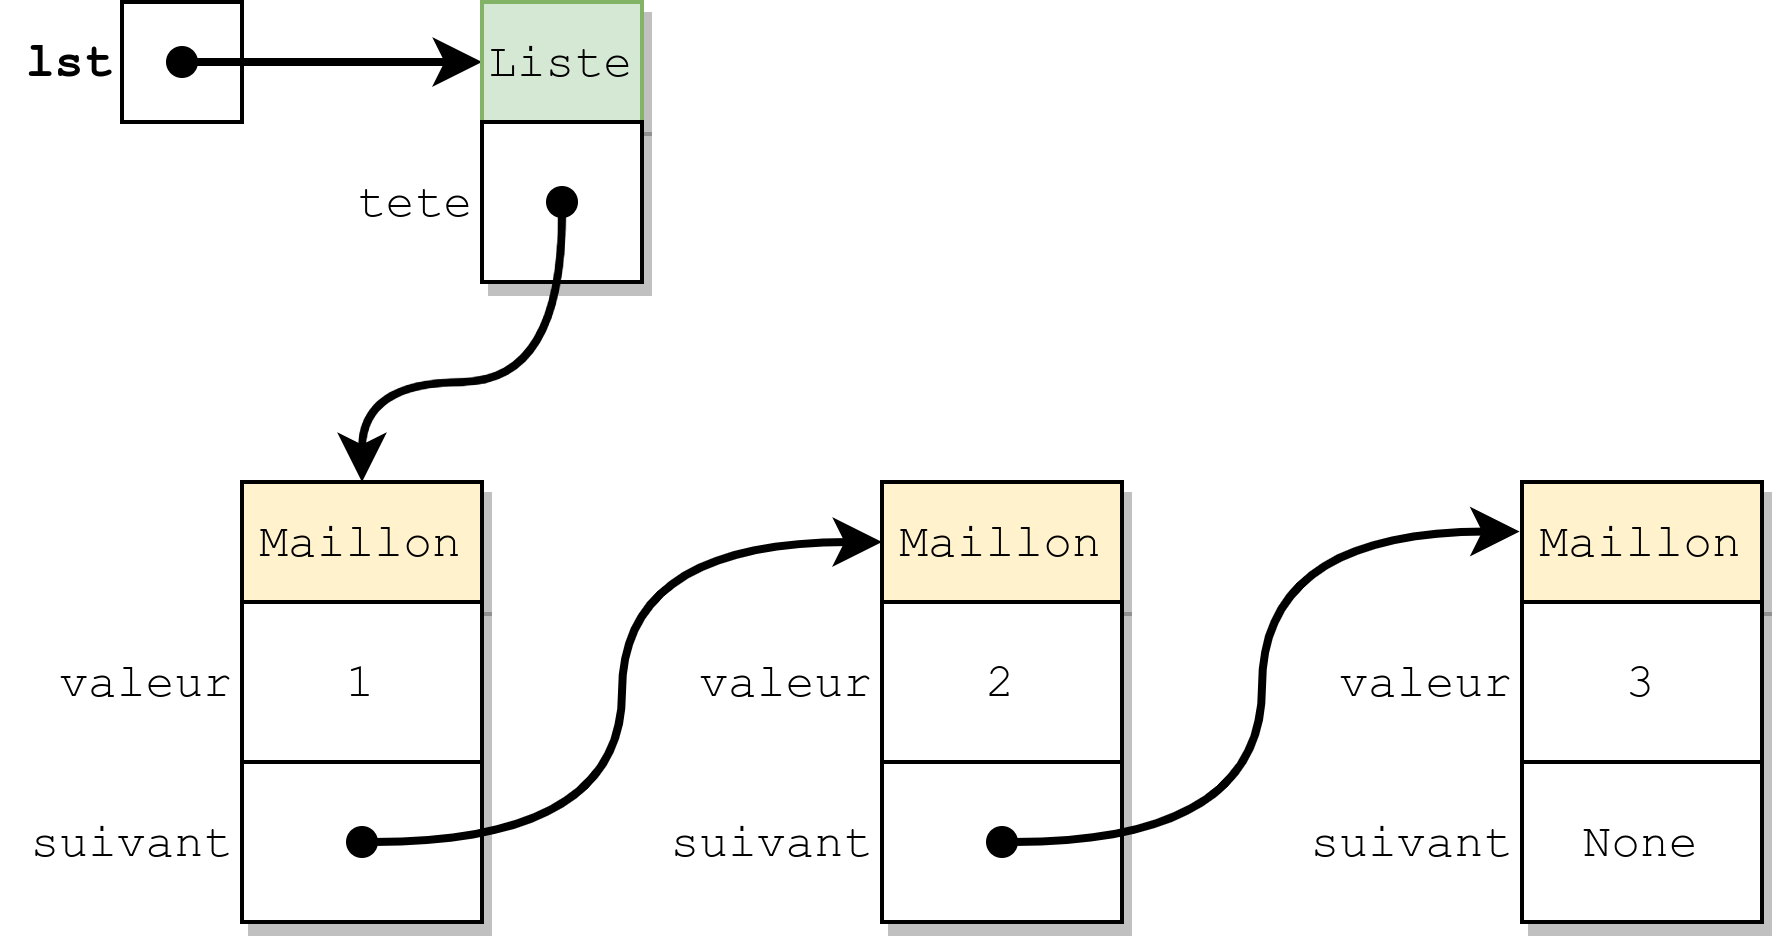
\includegraphics{maillon5.png}

On a donc construit ainsi la liste 1, 2, 3, dans cet ordre.
\begin{eleve}
    Implémenter dans la classe \texttt{Liste} la méthode \texttt{ajoute}
ayant un paramètre \texttt{valeur}. Cette méthode ajoute un nouveau
maillon en tête de la liste ayant pour valeur : \texttt{valeur} et pour
attribut \texttt{suivant} : l'ancien attribut \texttt{tete} de la liste.

Exemples :

\begin{verbatim}
>>> lst = Liste()
>>> lst.ajoute(1)
>>> print(lst.tete.valeur)
1
>>> lst.ajoute(2)
>>> print(lst.tete.valeur)
2
>>> print(lst.tete.suivant.valeur)
1
\end{verbatim}
        
        \end{eleve}
        {\scriptsize
    \begin{tcolorbox}[breakable, size=fbox, boxrule=1pt, pad at break*=1mm,colback=cellbackground, colframe=cellborder]
\prompt{In}{incolor}{ }{\boxspacing}
\begin{Verbatim}[commandchars=\\\{\}]
\PY{k}{class} \PY{n+nc}{Liste}\PY{p}{(}\PY{n}{Liste}\PY{p}{)}\PY{p}{:}
    \PY{k}{def} \PY{n+nf}{ajoute}\PY{p}{(}\PY{n+nb+bp}{self}\PY{p}{,} \PY{n}{valeur}\PY{p}{)}\PY{p}{:}
        \PY{l+s+sd}{\PYZdq{}\PYZdq{}\PYZdq{}}
\PY{l+s+sd}{        Ajouter un nouveau maillon en tête de liste}

\PY{l+s+sd}{        Args:}
\PY{l+s+sd}{            valeur (type): valeur du nouveau maillon}

\PY{l+s+sd}{        Exemples :}
\PY{l+s+sd}{        \PYZgt{}\PYZgt{}\PYZgt{} lst = Liste()}
\PY{l+s+sd}{        \PYZgt{}\PYZgt{}\PYZgt{} lst.ajoute(1)}
\PY{l+s+sd}{        \PYZgt{}\PYZgt{}\PYZgt{} print(lst.tete.valeur)}
\PY{l+s+sd}{        1}
\PY{l+s+sd}{        \PYZgt{}\PYZgt{}\PYZgt{} lst.ajoute(2)}
\PY{l+s+sd}{        \PYZgt{}\PYZgt{}\PYZgt{} print(lst.tete.valeur)}
\PY{l+s+sd}{        2}
\PY{l+s+sd}{        \PYZgt{}\PYZgt{}\PYZgt{} print(lst.tete.suivant.valeur)}
\PY{l+s+sd}{        1}
\PY{l+s+sd}{        \PYZdq{}\PYZdq{}\PYZdq{}}
        \PY{n+nb+bp}{self}\PY{o}{.}\PY{n}{tete} \PY{o}{=} \PY{n}{Maillon}\PY{p}{(}\PY{n}{valeur}\PY{p}{,} \PY{n+nb+bp}{self}\PY{o}{.}\PY{n}{tete}\PY{p}{)}


\PY{n}{testmod}\PY{p}{(}\PY{p}{)}
\end{Verbatim}
\end{tcolorbox}
    }

    \hypertarget{autres-muxe9thodes}{%
\subsubsection{Autres méthodes}\label{autres-muxe9thodes}}

    On peut maintenant reformuler nos opérations, à savoir
\texttt{longueur}, \texttt{nieme\_element}, \texttt{concatener} ou
encore \texttt{renverser}, comme autant de méthodes de la classe
\texttt{Liste}. Ainsi, on peut écrire par exemple la méthode
\texttt{longueur} qui nous permet d'écrire \texttt{lst.longueur()} pour
obtenir la longueur de la liste \texttt{lst}.

        {\scriptsize
    \begin{tcolorbox}[breakable, size=fbox, boxrule=1pt, pad at break*=1mm,colback=cellbackground, colframe=cellborder]
\prompt{In}{incolor}{ }{\boxspacing}
\begin{Verbatim}[commandchars=\\\{\}]
\PY{c+c1}{\PYZsh{} il faut importer la fonction `longueur`}
\PY{c+c1}{\PYZsh{} d\PYZsq{}une liste chaînée (cf. partie 3 du cours)}
\PY{k+kn}{from} \PY{n+nn}{operations\PYZus{}base} \PY{k+kn}{import} \PY{n}{longueur}


\PY{k}{class} \PY{n+nc}{Liste}\PY{p}{(}\PY{n}{Liste}\PY{p}{)}\PY{p}{:}
    \PY{k}{def} \PY{n+nf}{longueur}\PY{p}{(}\PY{n+nb+bp}{self}\PY{p}{)} \PY{o}{\PYZhy{}}\PY{o}{\PYZgt{}} \PY{n+nb}{int}\PY{p}{:}
        \PY{l+s+sd}{\PYZdq{}\PYZdq{}\PYZdq{}}
\PY{l+s+sd}{        Longueur d\PYZsq{}une liste chaînée}

\PY{l+s+sd}{        Returns:}
\PY{l+s+sd}{            int: longueur de la liste}

\PY{l+s+sd}{        Exemples:}
\PY{l+s+sd}{        \PYZgt{}\PYZgt{}\PYZgt{} lst = Liste()}
\PY{l+s+sd}{        \PYZgt{}\PYZgt{}\PYZgt{} assert lst.longueur() == 0}
\PY{l+s+sd}{        \PYZgt{}\PYZgt{}\PYZgt{} lst.ajoute(4)}
\PY{l+s+sd}{        \PYZgt{}\PYZgt{}\PYZgt{} assert lst.longueur() == 1}
\PY{l+s+sd}{        \PYZgt{}\PYZgt{}\PYZgt{} lst.ajoute(2)}
\PY{l+s+sd}{        \PYZgt{}\PYZgt{}\PYZgt{} assert lst.longueur() == 2}
\PY{l+s+sd}{        \PYZgt{}\PYZgt{}\PYZgt{} lst.ajoute(1)}
\PY{l+s+sd}{        \PYZgt{}\PYZgt{}\PYZgt{} assert lst.longueur() == 3}
\PY{l+s+sd}{        \PYZdq{}\PYZdq{}\PYZdq{}}
        \PY{k}{return} \PY{n}{longueur}\PY{p}{(}\PY{n+nb+bp}{self}\PY{o}{.}\PY{n}{tete}\PY{p}{)}


\PY{n}{testmod}\PY{p}{(}\PY{p}{)}
\end{Verbatim}
\end{tcolorbox}
    }
\begin{remarque}
    Il est important de noter qu'il n'y a pas confusion ici entre la
fonction \texttt{longueur} définie précédemment et la méthode
\texttt{longueur}. En particulier, la seconde est définie en appelant la
première. Le langage Python est ainsi fait que, lorsqu'on écrit
\texttt{longueur(self.tete)}, il ne s'agit pas d'un appel récursif à la
méthode \texttt{longueur} (un appel récursif s'écrirait
\texttt{self.longueur()}).

\texttt{longueur()} et \texttt{self.longueur()} sont deux fonctions
différentes !

        \end{remarque}
    On peut donner à cette méthode le nom \texttt{\_\_len\_\_} et Python
nous permet alors d'écrire \texttt{len(lst)} comme pour un tableau. En
effet, lorsque l'on écrit \texttt{len(e)} en Python, ce n'est qu'un
synonyme pour l'appel de méthode \texttt{e.\_\_len\_\_()}.

        {\scriptsize
    \begin{tcolorbox}[breakable, size=fbox, boxrule=1pt, pad at break*=1mm,colback=cellbackground, colframe=cellborder]
\prompt{In}{incolor}{ }{\boxspacing}
\begin{Verbatim}[commandchars=\\\{\}]
\PY{c+c1}{\PYZsh{} il faut importer la fonction `longueur`}
\PY{c+c1}{\PYZsh{} d\PYZsq{}une liste chaînée (cf. partie 3 du cours)}
\PY{k+kn}{from} \PY{n+nn}{operations\PYZus{}base} \PY{k+kn}{import} \PY{n}{longueur}


\PY{c+c1}{\PYZsh{} étendre la classe Liste pour ajouter des méthodes}
\PY{k}{class} \PY{n+nc}{Liste}\PY{p}{(}\PY{n}{Liste}\PY{p}{)}\PY{p}{:}

    \PY{k}{def} \PY{n+nf+fm}{\PYZus{}\PYZus{}len\PYZus{}\PYZus{}}\PY{p}{(}\PY{n+nb+bp}{self}\PY{p}{)}\PY{p}{:}
        \PY{l+s+sd}{\PYZdq{}\PYZdq{}\PYZdq{}}
\PY{l+s+sd}{        Permet d\PYZsq{}utiliser :}
\PY{l+s+sd}{            \PYZhy{} la fonction len avec les Liste}
\PY{l+s+sd}{            \PYZhy{} une instance de Liste comme une expression booléenne :}
\PY{l+s+sd}{                True  si et seulement si l\PYZsq{}instance est de longueur \PYZgt{} 0}
\PY{l+s+sd}{                False si et seulement si l\PYZsq{}instance est de longueur nulle}

\PY{l+s+sd}{        Exemples:}
\PY{l+s+sd}{        \PYZgt{}\PYZgt{}\PYZgt{} lst = Liste()}
\PY{l+s+sd}{        \PYZgt{}\PYZgt{}\PYZgt{} assert len(lst) == 0}
\PY{l+s+sd}{        \PYZgt{}\PYZgt{}\PYZgt{} if lst: print(\PYZdq{}expression booléenne évaluée à False\PYZdq{})}
\PY{l+s+sd}{        \PYZgt{}\PYZgt{}\PYZgt{} lst.ajoute(4)}
\PY{l+s+sd}{        \PYZgt{}\PYZgt{}\PYZgt{} assert len(lst) == 1}
\PY{l+s+sd}{        \PYZgt{}\PYZgt{}\PYZgt{} if lst: print(\PYZdq{}expression booléenne évaluée à True\PYZdq{})}
\PY{l+s+sd}{        expression booléenne évaluée à True}
\PY{l+s+sd}{        \PYZdq{}\PYZdq{}\PYZdq{}}
        \PY{k}{return} \PY{n}{longueur}\PY{p}{(}\PY{n+nb+bp}{self}\PY{o}{.}\PY{n}{tete}\PY{p}{)}


\PY{n}{testmod}\PY{p}{(}\PY{p}{)}
\end{Verbatim}
\end{tcolorbox}
    }

    De même, on peut ajouter à la classe \texttt{Liste} une méthode pour
accéder au n-ième élément de la liste, c'est-à-dire une méthode qui va
appeler notre fonction \texttt{nieme\_element} sur \texttt{self.tete}.
Le nom de la méthode est arbitraire et nous pourrions choisir de
conserver le nom \texttt{nieme\_element}. Mais là encore nous pouvons
faire le choix d'un nom idiomatique en Python, à savoir
\texttt{\_\_getitem\_\_}.

Ceci nous permet alors d'écrire \texttt{lst{[}i{]}} pour accéder au
i-ième élément de notre liste, exactement comme pour les tableaux.
\begin{eleve}
    Implémenter dans la classe \texttt{Liste} la méthode
\texttt{\_\_getitem\_\_} de paramètre \texttt{index} permettant de
renvoyer la valeur du maillon de rang \texttt{index} de la liste.
Utiliser pour cela la fonction \texttt{nieme\_element()}.

Exemple:

\begin{verbatim}
>>> lst = Liste()
>>> lst.ajoute(4)
>>> lst.ajoute(2)
>>> lst.ajoute(1)
>>> assert lst[0] == 1
>>> assert lst[1] == 2
>>> assert lst[2] == 4
\end{verbatim}
        
        \end{eleve}
        {\scriptsize
    \begin{tcolorbox}[breakable, size=fbox, boxrule=1pt, pad at break*=1mm,colback=cellbackground, colframe=cellborder]
\prompt{In}{incolor}{ }{\boxspacing}
\begin{Verbatim}[commandchars=\\\{\}]
\PY{c+c1}{\PYZsh{} il faut importer la fonction `longueur`}
\PY{c+c1}{\PYZsh{} d\PYZsq{}une liste chaînée (cf. partie 3 du cours)}
\PY{k+kn}{from} \PY{n+nn}{operations\PYZus{}base} \PY{k+kn}{import} \PY{n}{nieme\PYZus{}element}


\PY{c+c1}{\PYZsh{} étendre la classe Liste pour ajouter des méthodes}
\PY{k}{class} \PY{n+nc}{Liste}\PY{p}{(}\PY{n}{Liste}\PY{p}{)}\PY{p}{:}

    \PY{k}{def} \PY{n+nf+fm}{\PYZus{}\PYZus{}getitem\PYZus{}\PYZus{}}\PY{p}{(}\PY{n+nb+bp}{self}\PY{p}{,} \PY{n}{index}\PY{p}{)}\PY{p}{:}
        \PY{l+s+sd}{\PYZdq{}\PYZdq{}\PYZdq{} Permet d\PYZsq{}utiliser la syntaxe des listes}

\PY{l+s+sd}{        Exemples:}
\PY{l+s+sd}{        \PYZgt{}\PYZgt{}\PYZgt{} lst = Liste()}
\PY{l+s+sd}{        \PYZgt{}\PYZgt{}\PYZgt{} lst.ajoute(4)}
\PY{l+s+sd}{        \PYZgt{}\PYZgt{}\PYZgt{} lst.ajoute(2)}
\PY{l+s+sd}{        \PYZgt{}\PYZgt{}\PYZgt{} lst.ajoute(1)}
\PY{l+s+sd}{        \PYZgt{}\PYZgt{}\PYZgt{} assert lst[0] == 1}
\PY{l+s+sd}{        \PYZgt{}\PYZgt{}\PYZgt{} assert lst[1] == 2}
\PY{l+s+sd}{        \PYZgt{}\PYZgt{}\PYZgt{} assert lst[2] == 4}
\PY{l+s+sd}{        \PYZdq{}\PYZdq{}\PYZdq{}}
        \PY{k}{return} \PY{n}{nieme\PYZus{}element}\PY{p}{(}\PY{n}{index}\PY{p}{,} \PY{n+nb+bp}{self}\PY{o}{.}\PY{n}{tete}\PY{p}{)}


\PY{n}{testmod}\PY{p}{(}\PY{p}{)}
\end{Verbatim}
\end{tcolorbox}
    }

    Pour la fonction \texttt{renverser}, on fait le choix de nommer la
méthode \texttt{reverse} car là encore c'est un nom qui existe déjà pour
les tableaux de Python.
\begin{eleve}
    Implémenter dans la classe \texttt{Liste} une méthode \texttt{reverse}
ne renvoie rien mais inverse l'ordre des maillons de la liste.

Exemple :

\begin{verbatim}
>>> lst = Liste()
>>> lst.ajoute(3)
>>> lst.ajoute(2)
>>> lst.ajoute(1)
>>> lst.reverse()
>>> assert lst[0] == 3
>>> assert lst[1] == 2
>>> assert lst[2] == 1
\end{verbatim}
        
        \end{eleve}
        {\scriptsize
    \begin{tcolorbox}[breakable, size=fbox, boxrule=1pt, pad at break*=1mm,colback=cellbackground, colframe=cellborder]
\prompt{In}{incolor}{ }{\boxspacing}
\begin{Verbatim}[commandchars=\\\{\}]
\PY{c+c1}{\PYZsh{} il faut importer la fonction `renverser`}
\PY{c+c1}{\PYZsh{} d\PYZsq{}une liste chaînée (cf. partie 3 du cours)}
\PY{k+kn}{from} \PY{n+nn}{operations\PYZus{}base} \PY{k+kn}{import} \PY{n}{renverser}


\PY{k}{class} \PY{n+nc}{Liste}\PY{p}{(}\PY{n}{Liste}\PY{p}{)}\PY{p}{:}
    \PY{k}{def} \PY{n+nf}{reverse}\PY{p}{(}\PY{n+nb+bp}{self}\PY{p}{)}\PY{p}{:}
        \PY{l+s+sd}{\PYZdq{}\PYZdq{}\PYZdq{}}
\PY{l+s+sd}{        Renverse la liste en place}

\PY{l+s+sd}{        Exemples:}
\PY{l+s+sd}{        \PYZgt{}\PYZgt{}\PYZgt{} lst = Liste()}
\PY{l+s+sd}{        \PYZgt{}\PYZgt{}\PYZgt{} lst.ajoute(3)}
\PY{l+s+sd}{        \PYZgt{}\PYZgt{}\PYZgt{} lst.ajoute(2)}
\PY{l+s+sd}{        \PYZgt{}\PYZgt{}\PYZgt{} lst.ajoute(1)}
\PY{l+s+sd}{        \PYZgt{}\PYZgt{}\PYZgt{} lst.reverse()}
\PY{l+s+sd}{        \PYZgt{}\PYZgt{}\PYZgt{} assert lst[0] == 3}
\PY{l+s+sd}{        \PYZgt{}\PYZgt{}\PYZgt{} assert lst[1] == 2}
\PY{l+s+sd}{        \PYZgt{}\PYZgt{}\PYZgt{} assert lst[2] == 1}
\PY{l+s+sd}{        \PYZdq{}\PYZdq{}\PYZdq{}}
        \PY{n+nb+bp}{self}\PY{o}{.}\PY{n}{tete} \PY{o}{=} \PY{n}{renverser}\PY{p}{(}\PY{n+nb+bp}{self}\PY{o}{.}\PY{n}{tete}\PY{p}{)}


\PY{n}{testmod}\PY{p}{(}\PY{p}{)}
\end{Verbatim}
\end{tcolorbox}
    }

    Enfin, le cas de la concaténation est plus subtil, car il s'agit de
renvoyer une nouvelle liste, c'est-à-dire un nouvel objet. On choisit
d'appeler la méthode \texttt{\_\_add\_\_}, qui correspond à la syntaxe
\texttt{+} de Python.
\begin{eleve}
    Implémenter la méthode \texttt{\_\_add\_\_} de paramètre
\texttt{autre\_liste} qui renvoie une nouvelle liste, résultat de la
concaténation de la liste actuelle et de \texttt{autre\_liste}.

Exemple :

\begin{verbatim}
>>> lst_1 = Liste()
>>> lst_1.ajoute(1)
>>> lst_2 = Liste()
>>> lst_2.ajoute(3)
>>> lst_2.ajoute(2)
>>> lst_3 = lst_1 + lst_2
>>> assert lst_3[0] == 1     # lst_3 concaténée !
>>> assert lst_3[1] == 2
>>> assert lst_3[2] == 3
\end{verbatim}
        
        \end{eleve}
        {\scriptsize
    \begin{tcolorbox}[breakable, size=fbox, boxrule=1pt, pad at break*=1mm,colback=cellbackground, colframe=cellborder]
\prompt{In}{incolor}{ }{\boxspacing}
\begin{Verbatim}[commandchars=\\\{\}]
\PY{c+c1}{\PYZsh{} il faut importer la fonction `concatener`}
\PY{c+c1}{\PYZsh{} d\PYZsq{}une liste chaînée (cf. partie 3 du cours)}
\PY{k+kn}{from} \PY{n+nn}{operations\PYZus{}base} \PY{k+kn}{import} \PY{n}{concatener}


\PY{c+c1}{\PYZsh{} étendre la classe Liste pour ajouter des méthodes}
\PY{k}{class} \PY{n+nc}{Liste}\PY{p}{(}\PY{n}{Liste}\PY{p}{)}\PY{p}{:}
    \PY{k}{def} \PY{n+nf+fm}{\PYZus{}\PYZus{}add\PYZus{}\PYZus{}}\PY{p}{(}\PY{n+nb+bp}{self}\PY{p}{,} \PY{n}{liste}\PY{p}{)}\PY{p}{:}
        \PY{l+s+sd}{\PYZdq{}\PYZdq{}\PYZdq{}}
\PY{l+s+sd}{        Permet d\PYZsq{}utiliser l\PYZsq{}opérateur + entre instances de Liste}

\PY{l+s+sd}{        Exemples:}
\PY{l+s+sd}{        \PYZgt{}\PYZgt{}\PYZgt{} lst\PYZus{}1 = Liste()}
\PY{l+s+sd}{        \PYZgt{}\PYZgt{}\PYZgt{} lst\PYZus{}1.ajoute(1)}
\PY{l+s+sd}{        \PYZgt{}\PYZgt{}\PYZgt{} lst\PYZus{}2 = Liste()}
\PY{l+s+sd}{        \PYZgt{}\PYZgt{}\PYZgt{} lst\PYZus{}2.ajoute(3)}
\PY{l+s+sd}{        \PYZgt{}\PYZgt{}\PYZgt{} lst\PYZus{}2.ajoute(2)}
\PY{l+s+sd}{        \PYZgt{}\PYZgt{}\PYZgt{} lst\PYZus{}3 = lst\PYZus{}1 + lst\PYZus{}2}
\PY{l+s+sd}{        \PYZgt{}\PYZgt{}\PYZgt{} assert lst\PYZus{}3[0] == 1     \PYZsh{} lst\PYZus{}3 concaténée !}
\PY{l+s+sd}{        \PYZgt{}\PYZgt{}\PYZgt{} assert lst\PYZus{}3[1] == 2}
\PY{l+s+sd}{        \PYZgt{}\PYZgt{}\PYZgt{} assert lst\PYZus{}3[2] == 3}
\PY{l+s+sd}{        \PYZdq{}\PYZdq{}\PYZdq{}}

        \PY{n}{concat} \PY{o}{=} \PY{n}{Liste}\PY{p}{(}\PY{p}{)}
        \PY{n}{concat}\PY{o}{.}\PY{n}{tete} \PY{o}{=} \PY{n}{concatener}\PY{p}{(}\PY{n+nb+bp}{self}\PY{o}{.}\PY{n}{tete}\PY{p}{,} \PY{n}{liste}\PY{o}{.}\PY{n}{tete}\PY{p}{)}
        \PY{k}{return} \PY{n}{concat}


\PY{n}{testmod}\PY{p}{(}\PY{p}{)}
\end{Verbatim}
\end{tcolorbox}
    }
\begin{retenir}
    Une liste chaînée est une structure de données pour représenter une
séquence finie d'éléments. Chaque élément est contenu dans un Maillon,
qui fournit par ailleurs un moyen d'accéder au maillon suivant. Les
opérations sur les listes chaînées se programment sous la forme de
parcours qui suivent ces liaisons, en utilisant une fonction récursive
ou une boucle.

        \end{retenir}

    % Add a bibliography block to the postdoc
    
    
    
\end{document}
